\begin{frame}{Proof Systems}

    \begin{definition}[Cook, Reckhow 79]
        Proof system for $L \Leftrightarrow$ poly-time algorithm
        $\Pi\colon \{0, 1\}^* \times \{0, 1\}^* \rightarrow \{0, 1\}$:
        \begin{itemize}
            \item (completeness) $x \in L \Rightarrow \exists w ~ \Pi(x, w) = 1$;
            \item (soundness) $\exists w ~ \Pi(x, w) = 1 \Rightarrow x \in L$.
        \end{itemize}
    \end{definition}

    \deftext{Resolution}: proof of $\varphi \coloneqq \bigwedge\limits_{i} C_i$ is a sequence of clauses
    $(D_1, D_2, D_3, \dots, D_{\ell})$:
    \pause
    
    \begin{minipage}{0.3\linewidth}
        \begin{itemize}
            \item $D_i \in \{C_i\}$;
                \pause
            \item $\frac{A \lor x ~~~~~ B \lor \bar{x}}{A \lor B}$, $D_i \coloneqq A \lor B$;
                \pause
            \item $D_{\ell} = \emptyset$.
        \end{itemize}
    \end{minipage}
    \pause
    \begin{minipage}{0.68\linewidth}
        \centering
        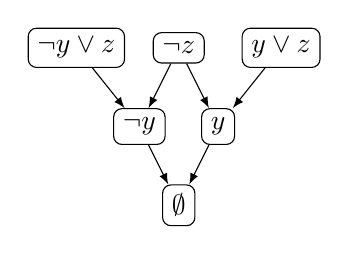
\begin{tikzpicture}[>=latex]
    \node[rectangle, rounded corners = 3pt, draw] (a) at (-1.3, 2)
        {$\neg y \lor z$};
    \node[rectangle, rounded corners = 3pt, draw] (a2) at (1.3, 2)
        {$y \lor z$};
    \node[rectangle, rounded corners = 3pt, draw] (b) at (0, 2)
        {$\neg z$};
    \node[rectangle, rounded corners = 3pt, draw] (c) at (-0.5, 1)
        {$\neg y$};
    \node[rectangle, rounded corners = 3pt, draw] (d) at (0.5, 1)
       {$y$};
    \node[rectangle, rounded corners = 3pt, draw] (e) at (0, 0)
        {$\emptyset$};

    \draw[->] (a) -- (c);
    \draw[->] (a2) -- (d);
    \draw[->] (b) -- (c);
    \draw[->] (b) -- (d);
    \draw[->] (c) -- (e);
    \draw[->] (d) -- (e);
\end{tikzpicture}
    \end{minipage}


    \pause
    \vspace{0.3cm}

    \deftext{Cutting Planes}: proof is a sequence of inequalities over $\mathbb{Z}$
    $(p_1 \ge 0, p_2 \ge 0, p_3 \ge 0, \dots, p_{\ell} \ge 0)$:
    \begin{itemize}
        \item $p_i$ is an encoding of $C \in \varphi$, $x_k \ge 0$ or $-x_k + 1 \ge 0$;
        \item $\frac{p_i ~~~~~ p_j}{p_k}$,  $(p_i \ge 0) \land (p_j \ge 0)$ imply $(p_k \ge 0)$
            \alert{over $\mathbb{Z}^n$};
        \item $p_{\ell} = 1$.
    \end{itemize}


\end{frame}


\begin{frame}{Pebbling}

    \begin{center}
        \tikzstyle{vert} = [
    circle,
    draw,
    inner sep = 0pt,
    minimum size = 0.45cm,
    fill = LEIorange!5
]
\tikzstyle{pstyle} = [alt = <{#1}>{fill = LEIorange!50}{}]
    
\tikzset{
    xcenter around/.style 2 args = {
        execute at end picture = {%
            \useasboundingbox let \p0 = (current bounding box.south west),
            \p1 = (current bounding box.north east),
            \p2 = (#1),
            \p3 = (#2) in ({min(\x2 + \x3 - \x1, \x0)}, \y0) rectangle ({max(\x3 + \x2 - \x0, \x1)},\y1);
        }
    }
}

\begin{tikzpicture}[xcenter around = {-2.1, -2.1}{2.1, 0.1}]
    \node at (3.6, -0.6) {
\includegraphics[scale = 0.09]{pics/utia-rest.png}};
    
    \node[vert, pstyle = 2, pstyle = {9-}, alt = <10>{fill = red!60}{}] (a) at (0, 0) {$r$};
    \node[vert, pstyle = 4, pstyle = {7-}] (b) at (-1, -1) {$x$};
    \node[vert, pstyle = {8-}] (c) at (1, -1) {$y$};
    \node[vert, pstyle = {3-4}, pstyle = {6-}] (d) at (-2, -2) {$z$};
    \node[vert, pstyle = {3-4}, pstyle = {6-}] (e) at (0, -2) {$u$};
    \node[vert, pstyle = 3, pstyle = {8-}] (f) at (2, -2) {$w$};

    \draw[->] (b) -- (a);
    \draw[->] (c) -- (a);
    \draw[->] (d) -- (b);
    \draw[->] (e) -- (b);
    \draw[->] (e) -- (c);
    \draw[->] (f) -- (c);
\end{tikzpicture}        
    \end{center}

    \pause
    \begin{itemize}
        \item $(\neg r)$;
            \pause
        \item $(z), (u), (w)$;
            \pause
        \item $(\neg z \lor \neg u \lor x), ~~ (\neg u \lor \neg w \lor y), ~~ (\neg x \lor \neg y \lor
            r)$.
    \end{itemize}

    \pause
    \tikzset{
    pr-vert/.style = {
        draw,
        rounded rectangle,
        minimum width = 1cm,
        minimum height = 0.4cm,
        outer sep = 0pt,
        fill = #1
    },
    pr-vert/.default = LEIblue!10
}

\tikzstyle{ops} = [alt = <{#1-}>{opacity = 1}{opacity = 0}]

\begin{tikzpicture}
    \node[pr-vert, ops = 6] (a) at (0, 0) {$u$};
    \node[pr-vert, ops = 6] (b) at (0, -1) {$z$};
    \node[pr-vert, ops = 6] (c) at (0, -2) {$\neg z \lor \neg u \lor x$};
    
    \node[pr-vert = LEIorange!10, ops = 7] (d) at (2, -1.9) {$\neg u \lor x$};
    \node[pr-vert = LEIorange!10, ops = 7] (e) at (3, -1.25) {$x$};

    \node[pr-vert, ops = 8] (f) at (4, 0) {$\neg u \lor \neg w \lor y$};
    \node[pr-vert, ops = 8] (g) at (6, 0) {$w$};
    
    \node[pr-vert = LEIorange!10, ops = 8] (h) at (5, -0.75) {$\neg w \lor y$};
    \node[pr-vert = LEIorange!10, ops = 8] (i) at (6.5, -1) {$y$};

    \node[pr-vert, ops = 9] (j) at (5, -2) {$\neg x \lor \neg y \lor r$};

    \node[pr-vert = LEIorange!10, ops = 9] (k) at (7.5, -2) {$\neg y \lor r$};
    \node[pr-vert = LEIorange!10, ops = 9] (l) at (8.5, -1.2) {$r$};

    \node[pr-vert, ops = 10] (m) at (8.5, 0) {$\neg r$};

    \node[pr-vert = red!30, ops = 10] (n) at (9.5, -0.6) {$\emptyset$};

    \draw[->, ops = 7] (b) -- (d);
    \draw[->, ops = 7] (c) -- (d);
    \draw[->, ops = 7] (a) -- (e);
    \draw[->, ops = 7] (d) -- (e);

    \draw[->, ops = 8] (a) -- (h);
    \draw[->, ops = 8] (f) -- (h);
    \draw[->, ops = 8] (h) -- (i);
    \draw[->, ops = 8] (g) -- (i);

    \draw[->, ops = 9] (e) -- (k);
    \draw[->, ops = 9] (j) -- (k);
    \draw[->, ops = 9] (k) -- (l);
    \draw[->, ops = 9] (i) -- (l);

    \draw[->, ops = 10] (l) -- (n);
    \draw[->, ops = 10] (m) -- (n);
\end{tikzpicture}
\end{frame}


\begin{frame}{Lower bounds in proof complexity}

    \tikzset{
    >=latex,
    perpinterface/.style = {
        postaction = {
            draw,
            decorate,
            decoration = {
                ticks,
                raise = 0.07cm,
                amplitude = 0.07cm,
                segment length = 1mm
            }
        }
    },
    % пружина
    vert/.style = {
        draw,
        ellipse
    },
    tikzart-fire/.pic = {
        \draw[fill = red!60] (0, 0) .. controls (0.3, 0) and (0.6, 0.1) .. (0.7, 0.3)
            .. controls (0.8, 0.5) and (0.85, 0.6) .. (0.8, 0.9)
            .. controls (0.75, 1.1) and (0.7, 1.2) .. (0.6, 1.4)
            .. controls (0.65, 1.2) and (0.6, 1.05) .. (0.5, 0.9)
            .. controls (0.5, 1.2) and (0.2, 1.3) .. (0.1, 1.6)
            .. controls (0.05, 1.75) and (0.1, 2) .. (0.2, 2.1)
            .. controls (-0.1, 2) and (-0.2, 1.85) .. (-0.3, 1.7)
            .. controls (-0.4, 1.5) and (-0.45, 1.3) .. (-0.4, 1.1)
            .. controls (-0.5, 1.2) and (-0.51, 1.4) .. (-0.5, 1.5)
            .. controls (-0.75, 1.2) and (-0.8, 0.7) .. (-0.7, 0.5)
            .. controls (-0.6, 0.28) and (-0.4, 0) .. (0, 0);
            \fill[white] (0, 0) .. controls (0.3, 0) and (0.52, 0.34) .. (0.37, 0.61)
            .. controls (0.4, 0.54) and (0.32, 0.32) .. (0.25, 0.25)
            .. controls (0.3, 0.35) and (0.25, 0.5) .. (0.2, 0.6)
            .. controls (0.1, 0.8) and (-0.05, 1) .. (0, 1.2)
            .. controls (-0.32, 1) and (-0.3, 0.72) .. (-0.2, 0.47)
            .. controls (-0.3, 0.51) and (-0.31, 0.6) .. (-0.33, 0.7)
            .. controls (-0.4, 0.6) and (-0.4, 0.5) .. (-0.4, 0.4)
            .. controls (-0.35, 0.18) and (-0.2, 0) .. (0, 0);
    }
}


    
\begin{tikzpicture}
    \node[vert] (res) at (1, 0) {$\Res$};
    \node[vert] (ns) at (-3, 0) {$\NS$};
    \node[vert] (cp) at (3, 1) {$\CP$};
    \node[vert] (acf) at (1.2, 1.5) {$\AC_0$-Frege};
    \node[vert] (resl) at (-1, 2.1) {$\ResL$};
    \node[vert] (acfp) at (0.5, 3.5) {$\AC_0[p]$-Frege};
    \node[vert] (fre) at (0.5, 5) {Frege};
    \node[vert] (ips) at (-2, 6) {$\PrSys{IPS}$};
    \node[vert] (pcr) at (-3, 2) {$\PCR[]$};
    \node[vert] (sos) at (-4, 2.5) {$\SOS$};

    \node[vert] (ns2) at (-5.5, 0) {$\NS_{\{\pm 1\}}$};
    \node[vert] (pcr2) at (-6, 2) {$\PCR[]_{\{\pm 1\}}$};
    \node[vert] (sos2) at (-6.8, 3) {$\SOS_{\{\pm 1\}}$};

    \node[vert] (cps) at (-4, 6.5) {$\PrSys{CPS}$};

    \draw[->] (res) -- (cp);
    \draw[->] (cp) to[out = 90, in = -20] (fre);
    \draw[->] (res) -- (resl);
    \draw[->] (res) -- (acf);
    \draw[->] (res) -- (pcr);
    \draw[->] (ns) -- (pcr);
    \draw[->] (resl) -- (acfp);
    \draw[->] (acf) -- (acfp);
    \draw[->] (acfp) -- (fre);
    \draw[->] (fre) -- (ips);
    \draw[->] (ips) -- (cps);

    \draw[->] (pcr) -- (ips);
    \draw[->] (sos) -- (cps);

    \draw[->] (ns2) -- (pcr2);
    \draw[->] (pcr2) -- (ips);
    \draw[->] (sos2) -- (cps);

    \node[inner sep = 0pt] at (-7, 5.5)
    {
\includegraphics[width = .2\textwidth]{pics/dragon.png}};

    \pause
    \draw[ultra thick, blue] (-4, -1) to[out = 110, in = 230] (-4.4, 3) to[out = 50, in = 180] (3.5, 1.8);
    \foreach \point in {(1.5, 3), (-2, 4), (-6, 1)}{
        \pic at \point {tikzart-fire};
    }
    
\end{tikzpicture}
\end{frame}

\begin{frame}{Hard formulas for all proof systems}

    \begin{itemize}
        \item If $\varphi$ is unsatisfiable then there is a ``proof'' of unsatisfiability.
            \pause
            \begin{itemize}
                \item \alert{And we can realize it in some proof system...}
            \end{itemize}
            \pause
        \item Distribution on formulas?
            \pause
            \begin{itemize}
                \item Fine. Counting argument do not work in proof complexity.
            \end{itemize}            
    \end{itemize}

    \pause

    \vspace{1cm}
    \begin{itemize}
        \item Random $\Delta$-CNF formulas
        \item Clique formulas
        \item Pseudorandom generator formulas
    \end{itemize}
\end{frame}


\begin{frame}{Random $\Delta$-CNF}

    \begin{minipage}{0.38\linewidth}
        \centering
        \begin{tikzpicture}

    \pgfmathsetseed{1000007}
    \foreach \i in {0, 1, ..., 5}{
        \node[graph-vert] (b\i) at
            (1.5, 0.4 * \i + 0.4) {};
    }

    \foreach \i in {0, 1, 3, 4, ..., 7}{
        \node[graph-vert = {LEIorange!80!black}{0.15cm}] (a\i) at
            (0, 0.4 * \i) {};

        \foreach \j in {0, 1, 2}{
            \pgfmathsetmacro{\temp}{random(0, 5)}
            \draw (a\i) -- (b\temp);
        }
    }

    \node[graph-vert, fill = green!50] (a2) at (0, 0.8) {};
    \foreach \j in {0, 1, 2}{
        \pgfmathsetmacro{\temp}{random(0, 5)}
        \draw[red, thick] (a2) -- (b\temp);
    }

    \node[below = 0.2cm] at (a0) {$m$};
    \node[below = 0.2cm] at (b0) {$n$};
\end{tikzpicture}
    \end{minipage}
    \begin{minipage}{0.58\linewidth}
        \begin{itemize}
            \item $m$ clauses;
            \item $n$ variables;
            \item $\Delta$ neighbours: $\binom{n}{\Delta}$ possibilities;
            \item negations (uniformly at random);
            \item $\mathfrak{D} \coloneqq \frac{m}{n}$ clause density.
        \end{itemize}
    \end{minipage}

    \pause
    \begin{itemize}
        \item $\mathfrak{D} > c_{\Delta} 2^{\Delta} \Rightarrow$ formula is unsat whp;
            \pause
        \item Fiege's conjecture: $\mathfrak{D} = \bigO{1} \Rightarrow$ no poly-time algorithm may
            ``prove'' unsatisfiability of random $\bigO{1}$-CNF.
            \begin{itemize}
                \item Non-approximability of many problems.
            \end{itemize}
    \end{itemize}

\end{frame}